\chapter{From Batch to Incremental 3D Reconstruction}

3D Reconstruction represents a long-standing topic of interest in both Computer Vision and Robotics communities. 
While Computer Vision aims at reconstructing an accurate and detailed model, leveraging on computationally intensive optimization methods, Robotics aims at rapidly understanding how the circumscribing world looks like, looking for the trade-off between accuracy and computational feasibility.
In recent years, the advances in the hardware capability, especially related to the powerful commodity graphics hardware (GPU-processing), and the design of efficient optimization algorithms, led Robotics and Computer Vision to become closer and closer in the 3D reconstruction (or mapping) field.
This chapter will give a comprehensive overview of both batch and incremental approaches to reconstruct the scene from a set or a sequence of images. We will focus in particular on the complex literature of Multi-View Stereo. This provides the basic of this thesis that aims at filling the gap between Structure from Motion/Simultaneous Localization and Mapping world and Multi-View Stereo itself. 

\minitoc


\section{Sparse Scene Structure Reconstruction and Camera Pose estimation}
\label{sec:slam}
Both Structure from Motion (SfM) in Computer Vision and Visual Simultaneous Localization and Mapping (V-SLAM) in Robotics face the problem of reconstructing a sparse map of the environment together with the pose (position and orientation) of the cameras that capture the scene.
Early researches of the two communities, focused on different aspects.
SfM aims at estimating accurately the map (structure) of a generic set of images, it has no particular time constraints and processes all the images in the same time (batch).
On the other hand, V-SLAM was thought to be deployed on a robot, therefore, the main goal is to obtain a fast and accurate estimate of the robot pose with respect to the environment by processing a video sequence: the SLAM algorithms needs to perform in real-time, \ie, at the same rate of the camera, and incrementally, \ie, a new image  has to be included in the estimation as soon as it becomes available.


These different approaches to the same problem, led the researchers of the two communities to develop deeply different algorithms which relies on different estimation tools.
Classical Structure from Motion algorithms \cite{triggs2000bundle,sibley2009adaptive,wu2011multicore} extract a set of 2D points for each image with a descriptor associated, such as SIFT \cite{sift} or ORB \cite{orb}, or others, then they find the correspondences of these 2D point among all the images that are likely generated by the same 3D point. Bootstrapping from an initial guess, SfM globally optimize the pose of the camera and the 3D points position, to minimize the error between the 2D points (the measurements) and the the projection of the current estimate of the 3D points on the cameras, i.e. the reprojection error, which is for instance represented by $e_r$ in Figure \ref{fig:reprojectionerror}.
If we deal with $n$ cameras, $k$ 3D points, we express $x_{ij}^{2D}$ the measurement of point $i$ in image $j$, and $\Pi_j(x_i^{3D})$ projects the 3D point $i$ on the image plane of the $j$-th camera, SfM aims at minimizing the following:
\[
\sum_{k}^{i=0}\sum_{n}^{j=0}||x_{ij}^{2D} - \Pi_j(x_i^{3D})||^2 = \sum_{k}^{i=0}\sum_{n}^{j=0}e_r(i,j) ^2.
\]
It is usually minimized by Gauss-Newton or Levenberg-Marquardt algorithms, and the process is named as Bundle Adjustment, since the minimization process adjusts the bundles of camera-to-point, by moving the camera poses and 3D point positions. This complete process requires a big computational effort.

\begin{figure}[t]
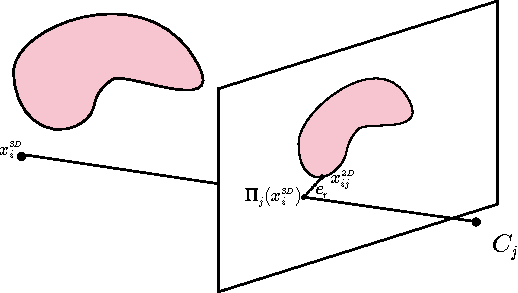
\includegraphics[width=0.99\columnwidth]{./img/ch_soa/reproj}
\label{fig:reprojectionerror}
 \caption{Reprojection error $e_r$ of 3D point $(x_i^{3D}$ in camera $j$.} 
\end{figure}



Instead, the SLAM approach \cite{davison2007monoslam,ceriani2014single,grasa2011ekf}, classically adopts a different point of view, focusing on the efficiency of the estimate, and so, it uses a different estimation tool, \ie, the Extended Kalman Filter (EKF) which estimates iteratively a state, composed by the camera pose with respect to the world together with the map of the environment, by incorporating the new measurement and marginalizing the old camera poses.  


Thanks to the Parallel Tracking and Mapping (PTAM) algorithm, proposed in \cite{klein_murray07}, these two approaches become closer and closer. PTAM proposed a SLAM system that adopts the bundle adjustment optimization: it decouples the fast tracking process, \ie, the camera pose estimation, and the slow mapping processes in two parallel thread.  
The tracking thread processes each frame of the video sequence while the mapping thread works only on keyframes. 
This new paradigm, named keyframe-SLAM, gains more and more interest in the robotics community, such that it becomes more popular with respect to the filtering approach \cite{strasdat2010real}.
Moreover, the improvements on the bundle adjustment optimization process proposed in \cite{kaess2008isam},  the formalization of the SLAM problem as a factor graph\cite{thrun2006graph}, and the optimization libraries g2o \cite{kummerle2011g} and GTSAM \cite{dellaert2012factor} led the researchers to move from the EKF estimation to keyframe-SLAM based on bundle adjustment \cite{strasdat11,sunderhauf2012towards,johannsson2013temporally}. 

% LSD-SLAM

In conclusion both SfM and SLAM algorithms are able to estimate the pose of the cameras and a point cloud representing the map of the environment: the former handles a generic set of data while the latter deals with a video sequence. 
In this thesis we rely on these points and cameras estimation and we provide a system able to handle a video sequence, or a set of subsequent images, that build a accurate, continuous and dense mesh map of the environment, exploiting the advances in Multi-View Stereo and incremental reconstruction from sparse points.

\section{Multi-View Stereo}


A wide literature in Computer Vision focuses on reconstructing a scene directly from the images by assuming that the camera poses are known, usually estimated by a Structure from Motion or SLAM algorithm.
These algorithms, known as Multi-View Stereo (MVS), aims at recovering a detailed dense and accurate reconstruction. 
While, SfM and SLAM algorithms output a sparse point cloud as a representation of the map of the environment, MVS reconstructs at least the big majority of the image pixels, resulting in a dense model of the environment.

%\subsection{Tools and Concepts}
Before a review of existing approaches  in Multi-View Stereo, we present some concepts that are common in almost all algorithms.

\subsection{Image appearance}
To understand how to compare different images to perform 3D reconstruction, we need to describe how each pixel of a single image is generated. 

The pixel intensity is proportional to the number of photons perceived by the camera sensor at that point, i.e., the amount of light that reaches it. This quantity, named \emph{irradiance}, is proportional to the \emph{radiance} of the scene which is the amount of light emitted by the objects.
For a surface patch in $x$, the radiance in direction $v$ is defined by the so called plenoptic function $L(x,v)$. 
The images are therefore a set of pixel whose value are observations of the plenoptic function.
This value is influenced by many factors: overall scene \emph{illumination}, \emph{reflectance} of the materials and the geometry of the objects perceived or how the camera sensor captures the light.

Since the estimation of the scene illumination is highly complex, in computer vision the illumination of the scene is represented by a point light sources.
The reflectance  is strictly related to the material of the surface;  if its value does not depend on time and wavelenght, and the material is exempt from scattering effects, the constant of proportionality between the reflected radiance and the irradiance of a surface is the bidirectional reflectance distribution function (BRDF) (see \cite{cohen2012radiosity}). 
%In Figure \todo{figure} 
The BRDF depends on the properties of the material, and capturing all the possible BRDF is not feasible in most cases. 
Therefore different BRDF models have been proposed and they generalize the reflectance different materials. 
In computer vision, and in the realm of Multi-View Stereo, the Lambertian model is usually adopted. It describes diffuse and smooth objects, whose radiance is independent to the point of view. 
According to this model, if a the light vector $\mathbf{l}$ is reflected by a surface with normal $\mathbf{n}$ and  constant albedo $\rho$, then the intensity of the radiance $L$ is 
\begin{equation}
  L = \rho \: \mathbf{n} \cdot \mathbf{l} = \rho \: |\mathbf{n}|  |\mathbf{l}| \: cos(\theta),
\end{equation}
where $\theta$ is the angle between $\mathbf{n}$ and $\mathbf{l}$ (see Figure \ref{fig:lamber}).

\begin{figure}[t]
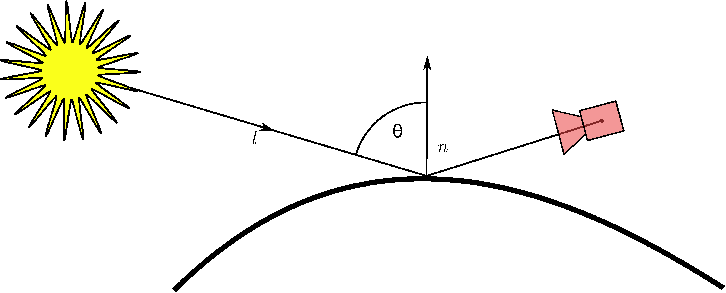
\includegraphics[width=0.99\columnwidth]{./img/ch_soa/lambert}
\label{fig:lamber}
 \caption{Lambertian model.} 
\end{figure}

In the real world almost no material is Lambertian, but the majority is close to Lambertian.
If we assume a point-wise light source in a Lambertian world, then, a 3D point projects on any camera to pixels with the same intensity, if this point is not occluded. 
Let $I_i$ and $I_j$ be two images, and $\Pi_i(x^{3D})$ and  $\Pi_j(x^{3D})$ the projections of the 3D point $x^{3D}$ in the two images, then:
\begin{equation}
 \label{eq:const_bright} 
 I_i(\Pi_i(x^{3D})) = I_j(\Pi_j(x^{3D})).
\end{equation}
This relation is the so called \emph{constant illumination assumption} which is widely exploited in computer vision, not only in Multi-View Stereo algorithms, but also in optical flow and in  any algorithm which pairwise comparison is needed.
Indeed, this assumption represents the basis to define photo-consistency measures.


\subsubsection{Photo-consistency}
Multi-View Stereo aims at recovering 3D information from a set of calibrated images. The coherence and accuracy measure to evaluate and optimize the recovered 3D data is called photo-consistency, which measures the similarity between two image regions.
Different photo-consistency measure have been proposed and they relies on the constant illumination assumption. 
Given images $I$ and $J$ and two pixels $p_0\in I$ and $q_0\in J$, a trivial photo-consistency measure is the difference between the intensity values  $I(p_0)$ and $J(q_0)$ but, taking into account only a single value, they lack in robustness. 
Robust photo-consistency measures consider a set of neighboring  pixels around $p_0$ and $q_0$, \ie, $p_i$ and $q_j$ where $1\leq i \leq n$ and $1\leq j \leq n$. Usually the neighboring pixels form a rectangular region; common measures are:
\begin{itemize}
  \item Sum of Squared Differences (SSD): $\sum_{i=0}^{n}(I(p_i) - J(q_i))^2$
  \item Sum of Absolute Differences (SAD): $\sum_{i=0}^{n}|I(p_i) - J(q_i)|$
  \item Normalized Cross-Correlation (NCC): $\frac{v_{I,J}(p_0,q_0)}{\sqrt{v_{I}(p_0) v_{J}(q_0)}}$,
  where 
  \begin{itemize}
    \item $v_{IJ}(p_0,q_0) = \frac{\sum_{i=0}^{n}I(p_i)J(q_i)}{n} - \mu_I(p_0) \mu_{J}(q_0)$
    \item $\mu_{I}(p_0) = \frac{\sum_{i=0}^{n}I(p_i)}{n}$ and $\mu_{J}(q_0) = \frac{\sum_{i=0}^{n}J(q_i)}{n}$ are the two mean values of the pixels considered in image $I$ and $J$
    \item $v_{I}(p_0) = \frac{\sum_{i=0}^{n}I(p_i)^2}{n} - \mu_I(p_0)^2$ and $v_{J}(q_0) = \frac{\sum_{i=0}^{n}J(q_i)^2}{n} - \mu_{J}(q_0)^2$ are the variances
  \end{itemize}
\end{itemize}
Low values of SSD and SAD represents high photo-consistency, while NCC is the correlation between two image regions, therefore high values corresponds to high photo-consistency. 
The computation of the NCC measure is more complex, but the final score is robust against linear illumination changes, and it partially compensates the limitation of the Lambertian model.


\subsection{Variational methods}
\label{subsec:variational}
In literature variational methods have been extensively adopted to reconstruct an accurate and photo-consistent model of the scene.
 They are widely used in the Computer Vision community, to solve an optimization problem involving an energy minimization.
Variational methods, also named  calculus of variations, aims at minimizing (or maximizing) a functional, \ie, a mapping $E$ from a vector space (each function $u$) to a real number. 
An example of general functional can be written as:
\begin{equation}
 E(u) = \int \mathit{L} (u, u')\;dx
\end{equation}
with $u'=\frac{du}{dx}$.
To minimize the functional $E$ we need to find its derivative with respect to the function $u$, through the Euler-Lagrange equation:
\begin{equation}
 \frac{\partial}{\partial u} \mathit{L} (u, u') - \frac{d}{dx} \frac{\partial}{\partial u'}\mathit{L} (u, u') =0
\end{equation}
The variational framework can be applied in Multi-View Stereo reconstruction \cite{hermosillo2002variational} as follows.

Given a set of images $\mathit{I}$ the functional $E$ usually writes as:
\begin{equation}
\label{eq:variational}
E(\mathit{u}) = E_{\text{data}}(\mathit{u}, \mathit{I}) + E_{\text{reg}} (\mathit{u})  
\end{equation}
where $E_{\text{data}}$  and $E_{\text{reg}}$ represent the data and the regularization terms, and function $\mathit{u}$ depends on the representation adopted for the 3D model of the scene.

In the surface evolution setting the function $\mathit{u}$ becomes the surface $\mathit{S}$ and the goal is to find the surface that minimizes the energy \eqref{eq:variational} usually written as:
\begin{equation}
 E(\mathit{S}) = \int_{\mathit{S}} g(\mathbf{x}, \mathbf{n}_{\mathit{S}}) \; ds  +\int_{\mathit{\Omega}} f(\mathbf{x}) \; d\mathbf{x}
\end{equation}
The function $\mathit{g}:\mathbb{R}^3\times\mathbb{S}^2 \rightarrow \mathbb{R}^+$ is named \emph{weighted area functional}  defined on the surface $\mathit{S}$ and represents the photo-consistency contribution to the total energy at point $\mathbf{x}$ with the associated normal $\mathbf{n}_{\mathit{S}}$.
The function $\mathit{f}$ is the so called \emph{ballooning} term and acts in the interior $\mathit{\Omega}$ of the surface $\mathit{S}$ as a potential that avoids the shrinkage to an empty surface (known as \emph{minimal surface bias}).

Gradient descent is a classical approach to minimize this energy, therefore Euler-Lagrange equation has to be applied in order to compute the gradient $\bigtriangledown E(\mathit{S})$ \cite{hermosillo2002variational}. Let $\mathit{S}^0$ be the initial surface and $\mathit{S}(t)$ the surface evolved at time $0$, then:
\begin{equation}
 \begin{cases}
  \mathit{S}(0) &=\mathit{S}^0\\
  \frac{\partial \mathit{S}(t)}{\partial t} & = -\bigtriangledown E(\mathit{S})
 \end{cases}
\end{equation}
Usually the two terms $E_{\text{data}}$ and $E_{\text{reg}}$ are threated separately since their meaning is deeply different.
The data term strictly depends on the representation of the model and the photo-consistency measure adopted, therefore we will provide more details in the following sections about shape representation. 
The regularization term is discussed in the following.
\subsection{Regularization}
In Multi-View Stereo, the reasons to enforce regularization are twofold. From a formal perspective, surface reconstruction can be described in a Bayesian point of view \cite[p. 11]{delaunoy2011modelisation}: the photo-consistency term represents only what we can infer from the observations (the images), instead the regularization represents the prior knowledge about the surface, \ie, the surface has to be smooth and regular. 
From a more practical point of view, images contains noise and the regularization term reduces the noise transferred in the reconstructed surface and it makes the optimization process more robust, \eg, by avoiding drifting degeneracies.

In the variational framework described thus far, regularization is achieved by minimizing the term $E_{\text{reg}}$. 
A common choice of this term lead the optimization to minimize the total area the surface, in order to obtain smooth solution:
\[
E_{\text{reg}} = \int_{\mathit{S}} ds.
\]
This choice biases the optimization to the minimal surface, and to avoid the empty surface solution the ballooning term described in previous section is adopted.

A more robust approach regularize the surface normals, by minimizing the following energy:
\[
E_{\text{reg}} = \int_{\mathit{S}} |\mathbf{n}(\mathbf{x}) - \mathbf{h}(\mathbf{x})|^2 ds
\]
where $\mathbf{n}(\mathbf{x})$ is the normal at point $\mathbf{x}$ and $\mathbf{h}(\mathbf{x})$ is the mean normal of the neighboring points of $\mathbf{x}$.

% \cite{li2015detail,heise2013pm,graber2015efficient}

A different approach to regularization relies on the Total Variation of the surface \cite{chambolle2010introduction}, \ie, 
\[
\int_{\mathit{\Omega}}|\bigtriangledown \mathit{S}|d\mathbf{x};
\]
we recall that  $\mathit{\Omega}$ is the interior of the surface $\mathit{S}$, and thanks to the absolute value operator, the functional is convex, therefore convex optimization methods may be applied.



\subsection{Shape Representations}
Since the datasets of \cite{seitz_et_al06} and \cite{strecha2008} were made available, dense MVS has been faced with different approaches, some of which reach very accurate results on these datasets.
It is hard to provide a unique classification of MVS algorithms since the methods proposed differ in many aspect, such as the input assumptions, the algorithm to obtain the reconstruction, optimization methods. 
Seitz \etal \cite{seitz_et_al06} proposed a subdivision according to the representation of the 3D model: \emph{depth maps}, \emph{volumetric},  \emph{level set} and \emph{mesh} methods. 
However Multi-View Stereo algorithms, especially the most complex and recent ones, often propose a pipeline requiring different representations of the scene.
% For instance depth maps-based algorithm needs a meshing step achieved by volumetric or implicit surfaces methods (level set).

\subsubsection{Depth Maps}
A depth map is a particular image that stores for each pixel the depth of the scene.
Usually the approaches based on this representation involve two steps: reference depth maps estimation and map merging.

Given a set of images, for each pixel $i$ of a reference image $I_{\text{ref}}$, the depth estimation aims at recovering the pixel depth, by pairwise comparing the appearance of the images. 
The basic idea is to look for the most likely depth $z_i$ generated from the $i$-th pixel of camera $C_i$ with respect to the image in camera $C_j$, as depicted in Figure \ref{fig:depth}.

A very popular approach, known as stereo matching \cite{scharstein2002taxonomy,lhuillier2002match}, compares two images as follows: for each pixel $i$ of the reference frame, it scans the corresponding epipolar line in the second image, and looks for the pixel whose neighboring patch best matches the patch around $i$ (see Figure \ref{fig:stereomatching}). 
Commonly used matching costs are the SSD (Sum of Squared Differences) or the NCC (Normalized Cross Correlation).
Some algorithms first rectify the two compared images, such that the epipolar line becomes horizontal and the scanning process becomes easier 
\cite{kang2001handling,bradley2008accurate,moons20093d}. 



\begin{figure}[t]
 \begin{tabular}{c}
  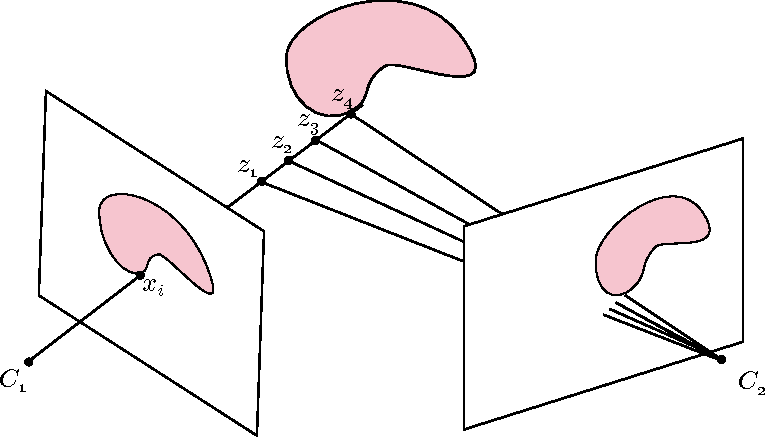
\includegraphics[width=0.98\columnwidth]{./img/ch_soa/depth}\\
 \end{tabular}
 \caption{Depth estimation process: the goal is to find the best depth corresponding to pixel $x_i$ of camera $C_i$, by comparison with other cameras.}
 \label{fig:depth}
\end{figure}


\begin{figure}[t]
 \begin{tabular}{c}
  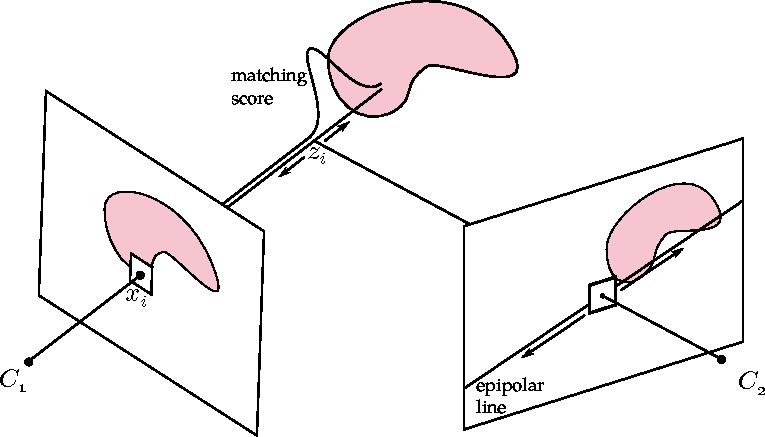
\includegraphics[width=0.98\columnwidth]{./img/ch_soa/stereomatching}\\
 \end{tabular}
 \caption{Stereo matching: the depth $z_i$ is estimated by comparing the appearance of the neighborhood of $x_i$ with the neighborhood of the pixels lying on the epipolar line in camera $C_2$.}
 \label{fig:stereomatching}
\end{figure}


Another approach named plane-sweeping \cite{collins1996space}, scans the entire 3D scene, that needs to be discretized, with a fronto-parallel plane, \ie, a plane parallel to the reference image plane where the other images are projected. 
For each pixel $i$ in the reference images, plane-sweeping compares the neighborhood patch against the corresponding patches in the set of projected images, and finally choose the depth $z_i$ corresponding to the best matching score. 
More recent approaches propose the usage of planes in multiple directions in the whole scene \cite{gallup2007real} or locally \cite{sinha2014efficient}
Space sweeping approaches compares the image with more accuracy with respect to the previous method, thanks to the 3D projection, but the computational effort is huge, even if highly parallelizable \cite{yang2003multi}.




\begin{figure}[t]
  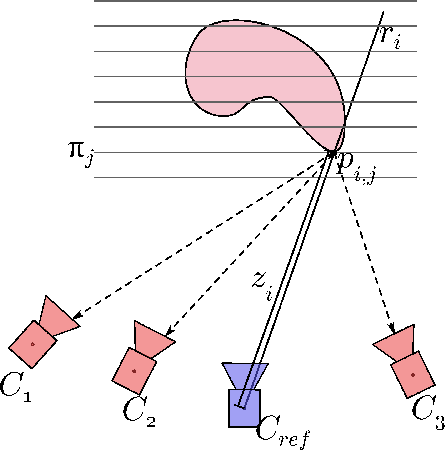
\includegraphics[width=0.9\columnwidth]{./img/ch_soa/planesweeping}
 \caption{Plane sweeping: the depth $z_i$ of point $p_{i,j}$ in the reference camera $C_ref$ is estimated by pairwise comparison of its projection to all the cameras.}
 \label{fig:planesweeping}
\end{figure}




The previous approaches outputs a noisy depth map that needs to be smoothed conveniently. 
A elegant approach to depth map estimation process aims at minimizing the energy:
\begin{equation}
 \label{eq:depthenergy} 
 E(z) = \sum_i \phi(z_i)  + \sum_{ij} \psi(z_i,z_j)
\end{equation}
that combines the function $\phi$ encoding the photo-consistency described in the previous approaches, and a function $\psi$ defined over the neighborhood of the pixel $i$ that penalizes differences to encode a smoothness prior. 
The minimization of this energy usually bootstraps from the noisy depth maps and leads to a more accurate and smooth set of depth maps.

Different optimization tools have been adopted to minimize Equation \eqref{eq:depthenergy}. In \cite{campbell2008using} the authors stores multiple hypothesis for each pixel depth, estimated with a classical stereo matching algorithm, then they optimize this initial depth map by modeling the problem as a Markov Random Field. Other optimization adopt graph-cuts \cite{kolmogorov2002multi} or Bayesian approaches \cite{strecha2006combined,gargallo2005bayesian} or propagation belief methods often referred as patch-based methods, since they usually estimate small oriented rectangular patches in 3D from seeded high accurate points to their neighborhood \cite{fu10,goesele2007multi,Tola12,bleyer2011patchmatch,heise2013pm}.




Some drawbacks affects this approach: the estimated depth maps are usually noisy; the depth of untextured regions are hard to model, such as the regions along the boundaries of occluded objects where the foreground objects corrupt the stereo matching process.
Some recent works address explicitly to these issues. 
In \cite{semerjian2014new} the authors estimate the depth maps as an energy minimization problem that aims at produce a edge-preserving smooth depth maps.
In \cite{wei2014multi} a coarse-to-fine approach together with propagation of the depth belief lead to clean depth maps.

Depth maps also model redundant information where a region is flat and each pixel of this planar region is estimated. 
Moreover a dense and continuous 3D model of the scene still needs to be reconstructed.

The subsequent step is therefore the fusion of the depth maps.
This step requires a 3D representation of the data,usually volumetric, that we describe in the following paragraphs, in which the input of the algorithms will often be a set of depth maps, or a point clouds estimated from the depth maps  as in \cite{curless1996volumetric} or directly through stereo matching techniques as in \cite{bradley2008accurate,labatut2007efficient,vu_et_al_2012}.

\subsubsection{Volumetric}
Many MVS algorithms model the scene from a point cloud, from a depth map or directly from images, by relying on a 3D discretization of the world space.
A sub-classification of these volumetric approaches considers how the space is discretized: with voxels or with tetrahedra.


\paragraph{Voxel-based}
A voxel is a the 3D extension of a pixel: if we partition the space in a regular 3D grid, each part, \ie, each small cube, is a voxel.
Voxel-based  algorithms are popular volumetric approach to merge depth maps or directly model from image, and performs very well in the Middelbury dataset \cite{seitz_et_al06}.

An early approach was proposed in \cite{curless1996volumetric} to integrate depth images into a single consistent model: it estimate a weighted signed distance function on the same volume from each depth map, it sums all of these volumes, and extracts a surface as the zero level set.
Goesele \etal \cite{goesele2006multi} extended this approach by reconstructing depth maps regions with an high accuracy.
Zach \etal \cite{zach2007globally} estimate a more robust distance function through total variation regularization with a $L^1$ norm data fidelity term.

Another very common approach, named  Poisson reconstruction \cite{kazhdan2006poisson}, creates a model out of the 3D oriented point associated with the depth maps: it computes an indicator function (defined as 1 at the points inside the model,and 0  outside) as a Poisson problem from a gradient field depending on the integral of the surface normal field.
An improvement on the Poisson Surface Reconstruction was recently proposed in \cite{shan2014occluding} where the internal contours estimated on the depth map, acts to densify the depth maps and, free space constraints computed for each voxels constrain the Poisson reconstruction in order to handle free space volumes.

A classical approach not requiring the depth map estimation, labels the voxels as free space or occupied, and is known as space carving or voxel coloring \cite{seitz1999photorealistic,kutulakos_seitz05} (see Figure \ref{fig:volumetric}). 
This method starts with a voxelized volume circumscribing the scene, and all voxels are initialized as occupied (or ``matter``). 
Low photo-consistent voxels are marked as free space iteratively, until a fixed photo-consistency threshold is reached. The boundary between free space and matter is therefore the final model of the scene. 
This method needs to take hard decision every time a voxel is classified, and highly depends on the order of inspection; the resulting reconstruction is often affected by artifacts and outliers.
An improvement was proposed in \cite{broadhurst2001probabilistic}, in which soft constraints are adopted to label more fairly the voxels.
Finally, the authors in \cite{yang2003multi} improve the order of inspection and adds a smoothing term. 
However the reconstruction of voxel-based space carving is still noisy and not  accurate.
Space carving, was also applied, more successfully by tetrahedron-based volumetric approach we will  review in next section.

More successful approaches to estimate a surface without depth maps, relies on global optimization of the energy \eqref{eq:variational} rewritten as:
\begin{equation}
\label{eq:eqVoxel}
E(\mathit{l}) = E_{\text{data}}(\mathit{l}) + E_{\text{reg}} (\mathit{l})  
\end{equation}
where $\mathit{l}:\mathit{P}\leftarrow \mathit{L}$ is the labeling function that associates a label $q\in \mathit{L}$ to the pixel $p \in\mathit{P}$, $E_{\text{data}}(\mathit{l})$ and $E_{\text{reg}} (\mathit{l})$ are related respectively to the photo-metric cost and the smoothness prior.

The most common optimization has been accomplished via graph cuts \cite{vogiatzis2005multi,kolmogorov2002multi,hornung2006hierarchical,furukawa2006carved,mucke2011surface,hernandez2007probabilistic}: the voxels are nodes of the graph, while the edges connect neighboring pixels and their capacity depends on the energy \eqref{eq:eqVoxel}. The boundary voxels links with the sink node of the graph, and voxels that are very likely to be inside the surface links to the source (see Figure \ref{fig:graphcut}).
These algorithms needs a ballooning term to avoid the shrinking bias, \ie, the minimization tends to traverse as few as possible edges and tends to extract an empty surface. If this term is too large, then the solution tends to over-inflate, otherwise the solution collapses into an empty surface.
This limitation has been partially solved in \cite{hernandez2007probabilistic} where the ballooning term depends  from the visibility, or in \cite{mucke2011surface} by replacing it with convenient weighting of the edges. 
Recently, convex optimization have been also successfully applied and reaches remarkable results
\cite{kolev2009continuous,kolev2010anisotropic,kostrikov2014probabilistic,savinov2016semantic}, they formalize the labeling problem as in the previous case, but compute the labels with the primal-dual method \cite{mehrotra1992implementation}.




\begin{figure}[t]
 \begin{tabular}{c}
  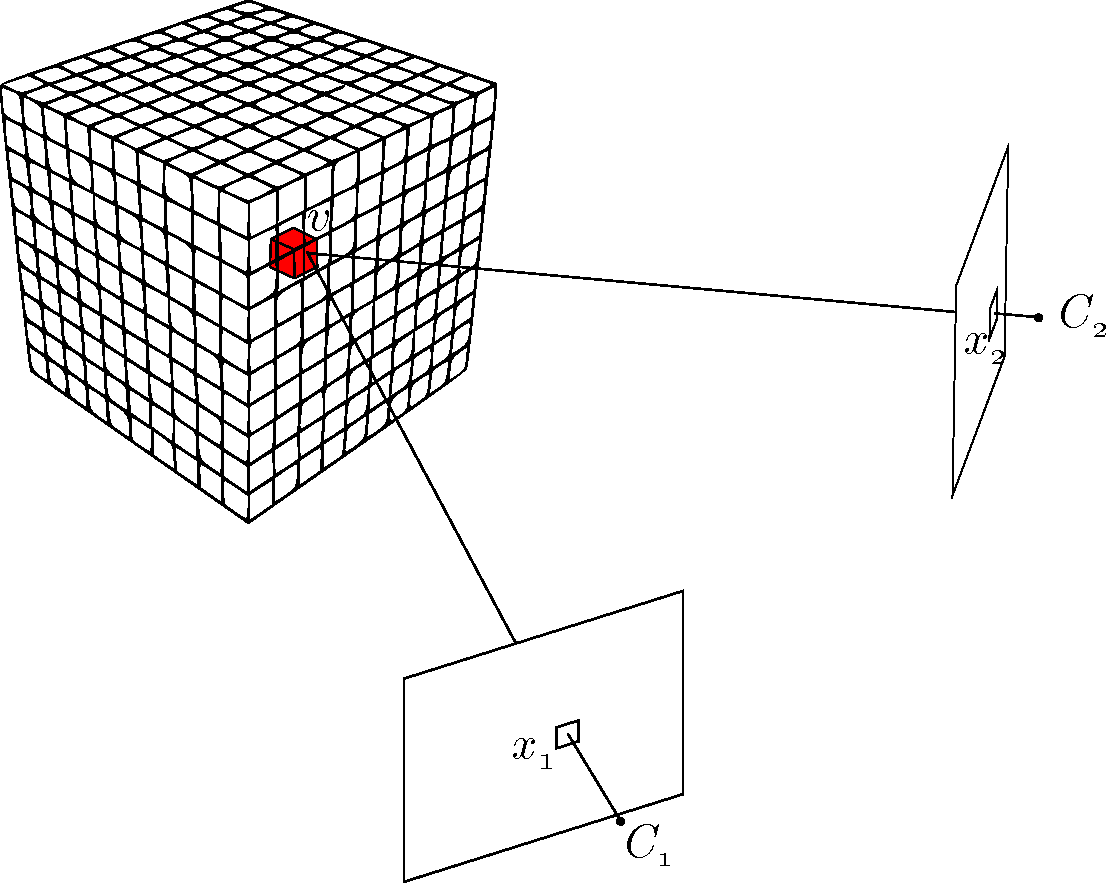
\includegraphics[width=0.98\columnwidth]{./img/ch_soa/volumetric}\\
 \end{tabular}
 \caption{Voxel coloring: the voxel $v$ is labelled as free or occupied according to its photo-consistency with respect to a set of pairwise cameras.}
 \label{fig:volumetric}
\end{figure}


In general, recent voxel-based methods yields accurate results, in particular when coupled with global optimization methods; however, their application is still limited by the huge requirement of memory, and even if attempts to make the representation more compact exist \cite{steinbrucker2014volumetric,chen2013scalable,zeng2013octree}, they are still not suitable for scalable large-scale reconstruction.
Moreover, only by including shape priors these methods are able to handle lack of texture \cite{karimi2015segment} that usually affects the depth maps.



\begin{figure}[t]
 \begin{tabular}{c}
  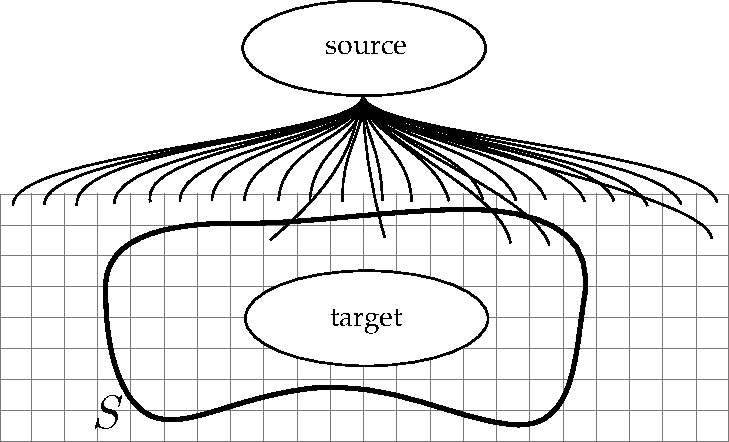
\includegraphics[width=0.98\columnwidth]{./img/ch_soa/graphcut}\\
 \end{tabular}
 \caption{Graph-cut reconstruction: bootstrapping from a discretion of the space, with the source node inside the surface, and the source node outside, this method look for the surfaces that cuts the graph according to a photo-consistency measure.}
 \label{fig:graphcut}
\end{figure}




\paragraph{Tetrahedron-based}
\label{sec:tet-based}
A different volumetric approach discretizes the space with a set of tetrahedra, usually computed via Delaunay Triangulation on a point cloud.
These methods are popular in the Computer Graphics community to reconstruct a surface from an unorganized (no adjacent among points is known) set of point \cite{amenta1999surface,amenta2001power,boissonnat1984geometric,dey2004provable,kolluri2004spectral}. 
Fewer tetrahedron-based methods with respect to the voxel-based ones, have been adopted in Multi-View Stereo reconstruction
\cite{faugeras_et_al_90,labatut2007efficient,salman2010surface,vu_et_al_2012,hiep2009towards,Pan_et_al09}.
They often rely on the space carving algorithm similar to the voxel coloring, but the boundary between free space and occupied parts is naturally a triangular mesh, very well-suited for further mesh refinement algorithms (see Figure \ref{fig:spacecarving} for a simple example of space carving in the 2D domain).




\begin{figure}[t]
 \begin{tabular}{cc}
  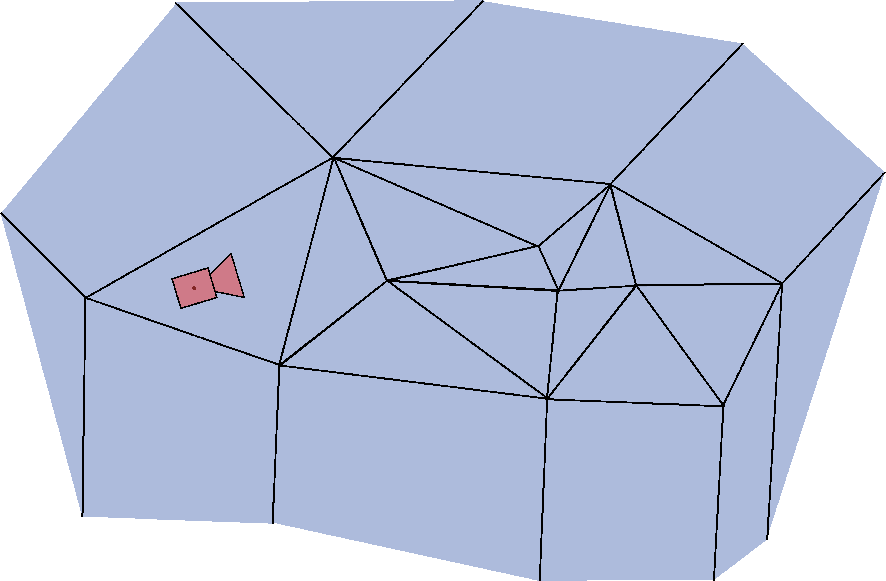
\includegraphics[width=0.48\columnwidth]{./img/ch_soa/spaceCarving01}&
  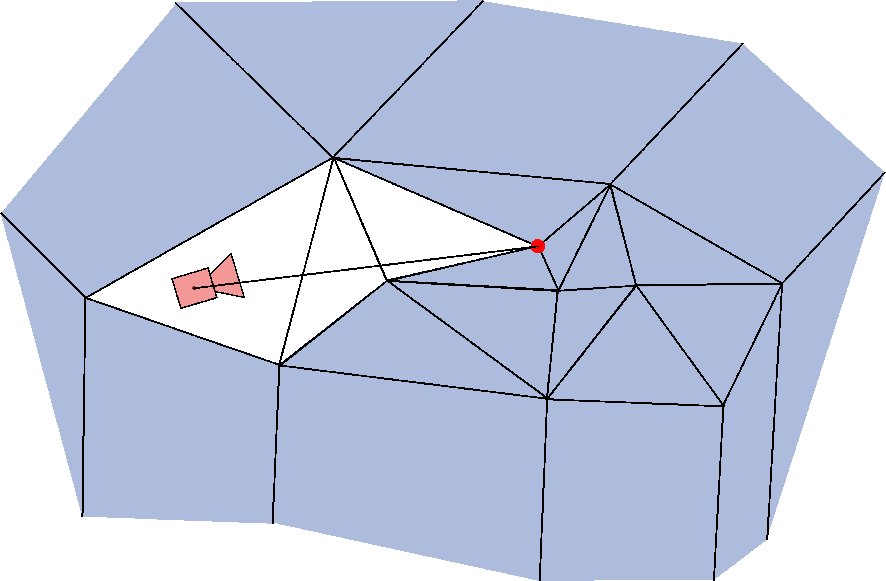
\includegraphics[width=0.48\columnwidth]{./img/ch_soa/spaceCarving02}\\
  (a) & (b)\\
 \end{tabular}
 \caption{Space carving in a triangulated space: (a) initialization with all ''matter`` tetrahedra, (b) carving performed by a camera-to-point visibility ray.}
 \label{fig:spacecarving}
\end{figure}


In the seminal work of Faugeras \etal \cite{faugeras_et_al_90} they apply a constrained Delaunay 3D triangulation to fit the stereo edges. They label  as free space the tetrahedra crossed by visibility rays from the camera to the edges as the space carving of the voxel-based approaches. The authors apply several times a region growing from not-labeled tetrahedra  until all not-labeled tetrahedra have been visited. Each iteration of each region growing keeps the boundary 2-manifold. Finally, each region is labeled as matter only if contains enough vertices, otherwise is free space. 
Even if this approach address the problem of reconstructing manifold surface, it does not handle genus greater than 0, \eg, a torus cannot be modeled, moreover the heuristic to label the tetrahedra is not robust to noise.


Labatut \etal \cite{labatut2007efficient} proposed to build the Delaunay triangulation upon a point cloud rich of points after the removal of redundant points. 
They extract the mesh of the model with the graph cut algorithm: they minimize an energy that takes into account photo-consistency and visibility. The results are scalable and accurate, but the final reconstruction heavily rely on the quality and distribution of the point cloud and it is not guaranteed to be 2-manifold.
In \cite{hiep2009towards} and \cite{vu_et_al_2012} the authors apply a similar approach but they subsequently optimize the mesh with a mesh evolution algorithm

ProForma \cite{Pan_et_al09} is an online reconstruction algorithm that tracks 2D features on the image frame by frame; their reconstruction performed every $k$ frames is added in a 3D Delaunay triangulation. They reconstruct a mesh through a probabilistic space carving approach. The approach works online for small objects, but scales poorly, since the triangulation and the reconstruction are re-executed for each keyframe.

In general, tetrahedron-based algorithms are volumetric methods  much more compact than voxel-based ones, but the accuracy of the reconstruction still needs a refinement to reach state-of-the-art results, indeed the output surface mesh is used as an initialization to mesh-based methods in \cite{vu_et_al_2012,hiep2009towards,salman2010surface}.

\subsubsection{Level set}
Level set methods define a model of the scene as the zero crossing of a function $f:\mathbf{R}^3\rightarrow\mathbf{R}$ \cite{faugeras2002variational,jin2002variational,yezzi2003stereoscopic,fuhrmann2014floating,solem2005geometric,yoon2010joint,pons2007multi}. 
They bootstrap the reconstruction from an initial surface and they evolve it by a variational approach which aims at minimize an energy functional.

For instance, in \cite{faugeras2002variational} the evolution of the surface, defined as zero crossing of $f$, is described by partial differential equation of the function $f$. A point on the surface moves proportionally to a value depending on the photo-consistency of its neighborhood: in particular, the more the neighbors are photo-consistent, the ore the point is near to zero.
The work in \cite{jin2002variational} extends this approach by managing surfaces with specular reflection thanks to a convenient choice of the pairwise cameras involved in the photo-consistency computation. In \cite{yoon2010joint} both the reflectiveness and the shape of the scene are estimated in the variational framework.
In both approaches the photometric measure is integrated in the 3D domain. In \cite{yezzi2003stereoscopic} the authors shows how the integration of this measure on the image domain produce more accurate results.

Solem \etal \cite{solem2005geometric} propose a geometric formalization of the variational minimization, in particular they replace the partial differential equation with the gradient, showing its robustness.
In \cite{pons2005modelling,pons2007multi} non rigid scene were reconstructed by including the motion in the optimizaton procedure.

A recent work of Fuhrmann \etal \cite{fuhrmann2014floating} proposes a new implicit function which integrates in the reconstruction process the points and their scale, \eg, the patch size, which may differ from one point to another. 


Level set methods lead to accurate results, handles implicitly topology changes, but often relies on a memory consumption volumetric initialization, and the evolution of the surface is not always easy to track and understand.


\begin{figure}[t]
\centering
 \begin{tabular}{c}
  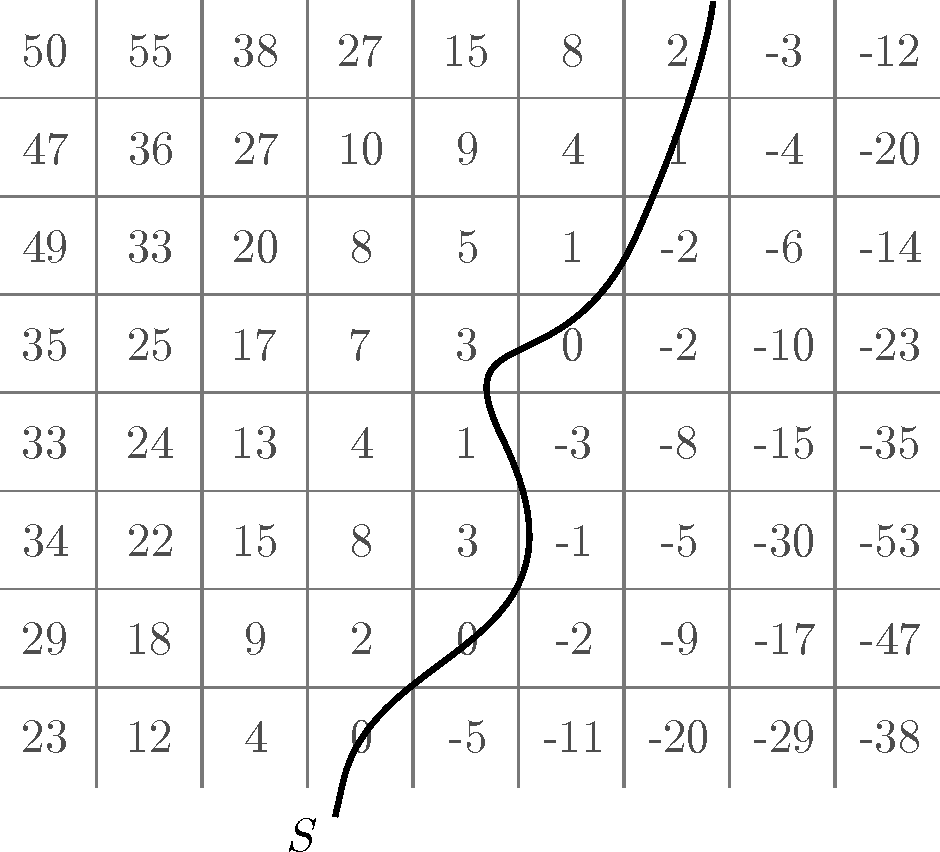
\includegraphics[width=0.48\columnwidth]{./img/ch_soa/levelset}\\
 \end{tabular}
 \caption{Level set reconstruction: the reconstruction is the zero-crossing surface of the function defined over the space (conveniently discretized).}
 \label{fig:levelset}
\end{figure}
\subsubsection{Mesh}

The last class of MVS algorithms represents the scene as a surface mesh. Some of the methods of the previous paragraphs outputs a mesh, but is always estimated from a different representation which play the major role in the reconstruction process.
The following methods, instead, deals directly with a mesh recovered from point clouds, depth maps or as a evolution of an initial mesh surface.

The early Mesh Zippering algorithm \cite{turk1994zippered} creates a triangular mesh from depth maps. It registers all the point clouds with a variant of the ICP (Iterative Closest Point); it creates a mesh for each depth map and finally merge all the meshes.

A mesh from depth images is directly estimated in \cite{pollefeys_et_al_08} too, by applying a coarse-to-fine approach for each depth camera: they bootstraps from a 3D rectangle mesh made up by two triangles that covers all the depth image, each triangle is subdivided and its position re-estimated whenever discontinuity or non-planarity in the depth map region enclosed in the triangle occurs. The meshes generated for each depth maps are registered thanks to the sensor calibration, and the redundant triangles are deleted.

Bradley \etal \cite{bradley2008accurate} propose to triangulate clusters of the point cloud estimated via depth maps, then estimate a mesh out of the triangulation and merge the sub maps created.

Generally, these algorithms estimates a mesh for each depth maps and merge the surfaces mesh to obtain a final model.

More direct approaches that avoids the mesh merging procedure, which may lead to artifacts relies on the volumetric approaches presented in \ref{sec:tet-based}.
For instance a big subset of mesh-based algorithms refine a coarse mesh of the scene, for instance the visual hull \cite{hiep2009towards,zaharescu2007transformesh,delaunoy_et_al_08,gargallo2007minimizing,delaunoy2011gradient,vu2011large}. These algorithms are similar to the level-set method but they directly evolve the mesh in 3D, without the need to extract the surface from an implicit function representation.
The methods proposed in \cite{delaunoy_et_al_08,gargallo2007minimizing,delaunoy2011gradient} evolve the surface to minimize the energy \eqref{eq:eqVoxel} rewriting the photo-consistency term for an image $I$ of camera $i$ as:
\begin{equation}
\label{eq:generative}
  E_{\text{data}}(S) = \int_{\mathit{I}} \rho\left(I(\mathit{u}), I^*_{\Omega}(\mathit{u})\right) d\mathit{u},
\end{equation}
where $\rho$ is a photo-consistency measure, $I$ is the image while $I^*$ is the current estimated surface and texture, rendered in camera $i$.
This equation integrates the photo-consistency in the image domain while most of other level set methods integrate this measure in the surface domain. This lead to more natural Bayesian formalization of the reconstruction. 
However, these approaches, named generative, have the drawback of not implicitly considering the occlusions which makes the functional difficult to be optimized. They need an explicit management of the visibility as in \cite{delaunoy2011gradient}.

A more straightforward approach to surface evolution was proposed by \cite{hiep2009towards} and \cite{vu2011large} which minimize an energy between pairwise images $i$ and $j$:
\begin{equation}
\label{eq:nongen}
  E_{\text{data}}(S) = \int_{\Omega^{\mathit{S}}_{ij}} \rho\left(I(\mathit{u}), I^{\mathit{S}}_{ij}(\mathit{u})\right) d\mathit{u}
\end{equation}
where the image $I^{\mathit{S}}_{ij}$ is the backprojection of the image of camera $j$ to camera $i$ through the current estimated surface $\mathit{S}$, \ie, $I^{\mathit{S}}_{ij} = I_j \circ \Pi_j \circ \Pi_i^{-1}$ , $\Omega^{\mathit{S}}_{ij}$ represent the domain of the surface where the reprojection is defined.

Both the approaches optimize the energies \eqref{eq:generative} and \eqref{eq:nongen} via gradient descent as described in Section \ref{subsec:variational}:

These mesh-based methods have proved to lead to very accurate results and  by estimating  sub-maps and then merge them together as in \cite{vu2011large},  large-scale reconstruction is feasible both on computational and memory sides.


\subsection{Initialization}
Most of the  multi-view algorithms presented thus far, especially the variational-based ones, bootstrap the optimization from an initial estimate of the 3D model; the initialization is a key point to reach accurate reconstructions.

A common and simple method to initialize MVS algorithm relies on the visual hull \cite{laurentini1994visual}. 
The visual hull is computed by removing the background pixels of each image and by intersecting the cones from the camera centers through the silhouettes Figure (\ref{fig:visualhull}). 
The output is an approximate model of the scene (Figure \ref{fig:visualhullex}(a) and \ref{fig:visualhullex}(c)), which however is computed very fast, and sufficiently close to the optimized solution (Figure \ref{fig:visualhullex}(b) and \ref{fig:visualhullex}(d)): these reasons lead the visual hull to become very popular in MVS literature \cite{jin2002variational,soatto2003tales,zaharescu2007transformesh,yoon2010joint}.

The visual hull requires the silhouettes of the captured object: they exist only if the images capture a single object, or a ver limited amount of objects.
In a generic scene, the silhouettes are very hard to compute or they neither exist.
A more general approach to initialize MVS algorithm builds a surface upon a point cloud estimated for instance via plane sweeping, Structure from Motion or by depth map estimation.
For instance Furukawa \etal \cite{fu10} estimate very reliable 3D points and expand their estimate in the neighborhood, finally they apply the Poisson Reconstruction. 
Labatut \etal \cite{labatut2007efficient} and Vu \etal \cite{vu_et_al_2012} build a Delaunay triangulation upon a very dense point cloud, by minimizing an energy functional via graph cuts.

Especially in surface evolution setting, a very desirable property for a robust initialization is the manifoldness, in order to avoid degeneracies in the optimization procedure. 
however, this issue has not be faced neither by \cite{fu10} and by \cite{labatut2007efficient,vu_et_al_2012}: both Poisson Reconstruction and graph cut may lead to non-manifoldness.

% \subsection{Shape priors}
% \subsection{Large Scale}

\begin{figure}[t]
\centering
 \begin{tabular}{cccc}
  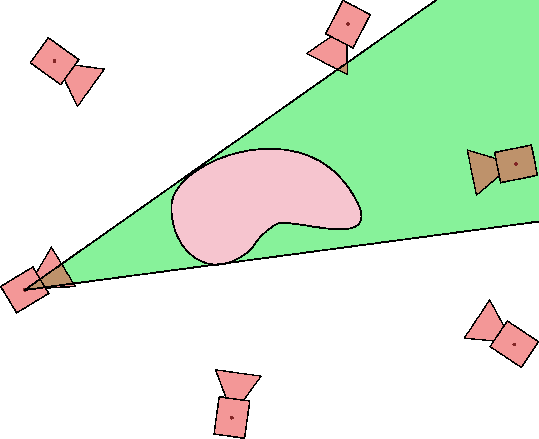
\includegraphics[width=0.45\columnwidth]{./img/ch_soa/visualhull01}&
  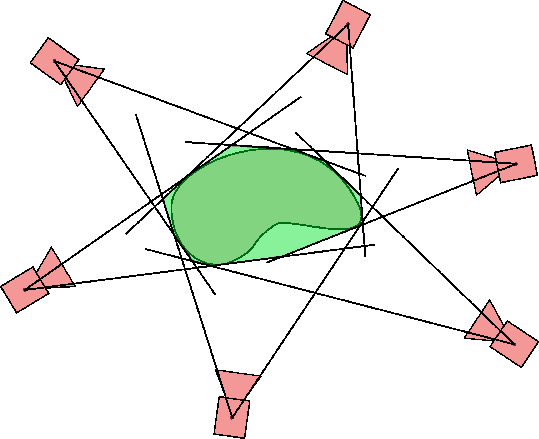
\includegraphics[width=0.45\columnwidth]{./img/ch_soa/visualhull02}\\
  (a)&(b)
 \end{tabular}
 \caption{Visual hull creation; in green: (a) the visual hull from the first camera; (b) the final visual hull.}
 \label{fig:visualhull}
\end{figure}

\begin{figure}[t]
\centering
 \begin{tabular}{cccc}
  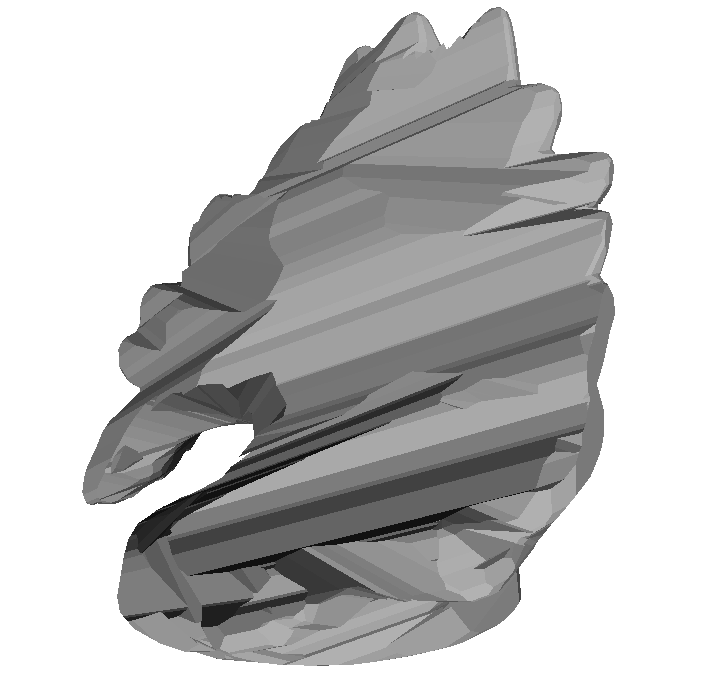
\includegraphics[width=0.24\columnwidth]{./img/ch_soa/dinoHull01}&
  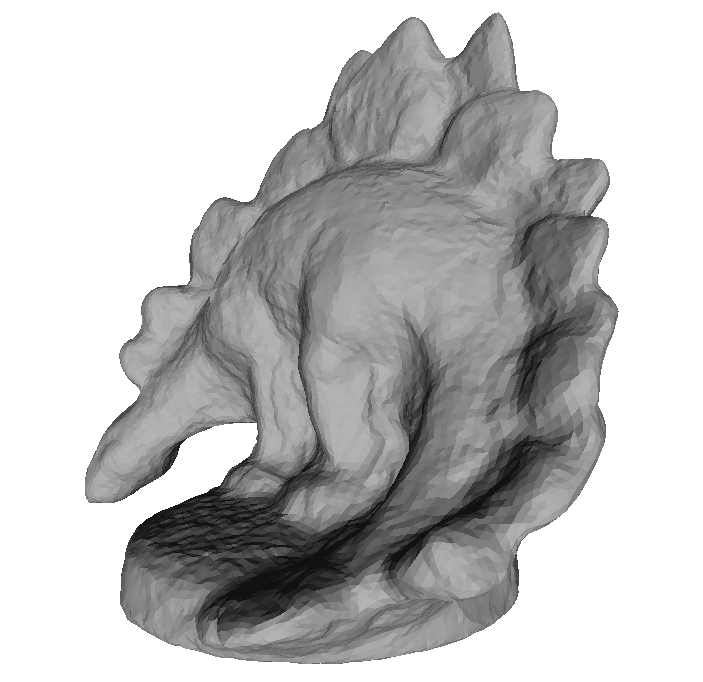
\includegraphics[width=0.24\columnwidth]{./img/ch_soa/dinoRef01}&
  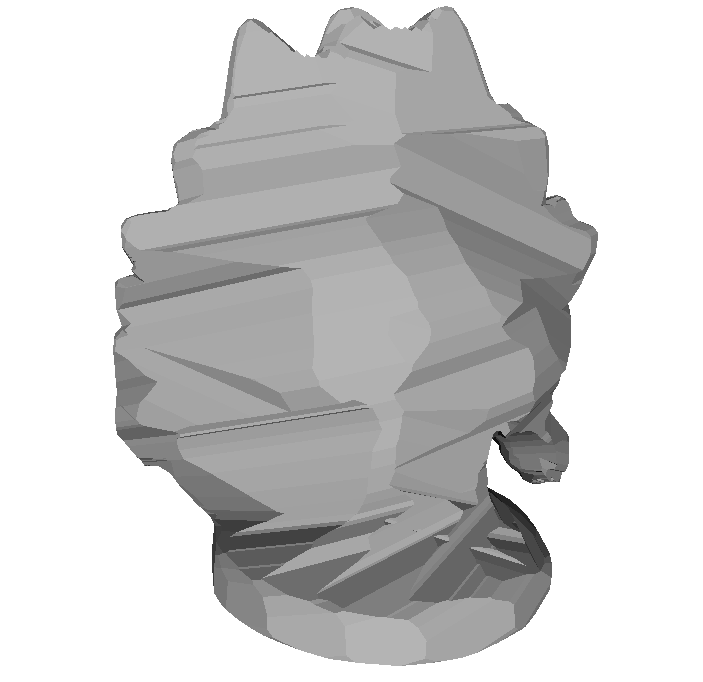
\includegraphics[width=0.24\columnwidth]{./img/ch_soa/dinoHull02}&
  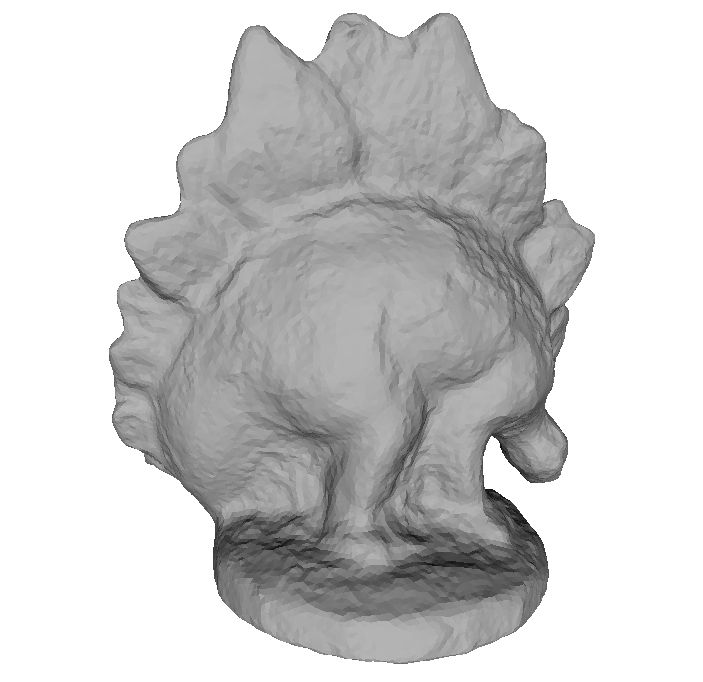
\includegraphics[width=0.24\columnwidth]{./img/ch_soa/dinoRef02}\\
  (a)&(b)&(c)&(d)
 \end{tabular}
 \caption{Example of visual hull (a) and its refinement (b) for the dinoSparse dataset \cite{seitz_et_al06}.}
 \label{fig:visualhullex}
\end{figure}
\section{Incremental reconstruction} 
The Multi-View Stereo algorithms described in the previous section are designed to be applied in a batch setting, \ie, the optimization process takes into account the whole set of images in the same time.
In some applications, especially in robotics, an incremental reconstruction algorithm is more suitable, for instance, for robot navigation, for traversability analysis, and for localization.
\subsection{Dense Simultaneous Localization and Mapping}
In Section \ref{sec:slam} we presented two approaches to reconstruct a sparse point cloud of the environment together with the camera trajectory and how the two problems become closer and closer: the optimization tool adopted in the batch algorithms of the classical structure from motion, became more and more common in the incremental SLAM algorithms \cite{mouragnon_et_al07,strasdat11}.

Similarly, since the proposals of Newcombe \etal \cite{newcombe2010live,newcombe2011kinectfusion,newcombe2011dtam} and St{\"u}ckler \etal \cite{stuhmer2010real}, Multi-View Stereo becomes closer to the robotics community: variational optimization on depth maps estimation and fusion has been performed in parallel with a camera tracking thread.

Newcombe \etal \cite{newcombe2010live} proposed to use structure from motion points and camera poses extracted incrementally by PTAM \cite{klein_murray07}, and to build an initial surface by interpolating the points with radial basis function as \cite{ohtake2003multi}; then by GPU dense optical flow, they estimate the difference between the predicted image with the initial surface and the observation (the images), to update the model.

KinectFusion \cite{newcombe2011kinectfusion} deals with RGB-D data, \ie, range data acquired  directly and coded in the images. It registers the points from the range data to the estimated surface, and updates  a volumetric Truncated Signed Distance Function (TSDF) according the data. DTAM \cite{newcombe2011dtam} extended the same approach to RGB by proposing a robust approach to estimate range data in real time exploiting the power of GPU processing.

Recently \cite{bylow2013real} improved the registration of RGB-D data of the KinectFusion approach by exploiting the information encoded in the TDSF, and \cite{concha2015incorporating} improved on DTAM by incorporating planar and layout priors in the estimation. The author in \cite{stuhmer2012parallel,stuckler2014multi} proposed different approaches to estimate and register depth maps in real time.

Most of the previous approaches rely on data from RGB-D cameras, not always available, for instance in outdoor environment; moreover they adopt depth map  volumetric representation that results to be not scalable for large-scale scenes.  

\subsection{Incremental reconstruction from sparse points}
A different class of incremental algorithms builds a dense model of the environment directly on the SfM points.
Incremental 3D reconstruction from a sparse point cloud is gaining interest in the computer vision community as incremental Structure from Motion algorithms are consolidating  \cite{wu13}, especially where GPU-demanding Dense SLAM methods cannot be applied. 
% This is clearly true for those applications where a rough, but dense, surface represents a sufficient and effective representation of the scene, e.g, for traversability analysis in unmanned vehicle navigation. 
% Furthermore, in real-time applications, the map of the environment needs to be updated online, and the surface has to be estimated incrementally. 

Most of the existing incremental algorithms \cite{lovi_et_al_11,Pan_et_al09,litvinov_lhuillier_13,litvinov_Lhiuller14} bootstrap the reconstruction of a mesh surface from the 3D Delaunay triangulation of a sparse point cloud. Indeed, the Delaunay property, \ie, no point of the triangulation is inside the sphere circumscribing any tetrahedron, avoids as much as possible the resulting tetrahedra to have a degenerate shape \cite{Maur_02}; it is self-adaptive, \ie, the more the points are dense the more the tetrahedra are small; it is very fast to compute, and to  update against point removal or addition; off-the-shelf libraries, such as CGAL \cite{cgal}, enable a very simple and efficient management of it. 

As soon as a Delaunay triangulation is available, several approaches exist to extract a surface taking into account the visibility of each point. 
We recall the simple space carving \cite{kutulakos_seitz05}: it initializes all the tetrahedra as \emph{matter}, then it marks as \emph{free space} the tetrahedra intersected by the camera-to-point \emph{viewing rays}, \ie, the lines from the camera center to the observed 3D points in the triangulation. 
The boundary between free space and matter represents the final surface of the scene.
Pan et al. \cite{Pan_et_al09} improve upon this simple procedure by proposing an online probabilistic Space Carving, but this is not an incremental approach: they start from scratch every time new points are added.
Lovi et al. \cite{lovi_et_al_11} present the first incremental Space Carving algorithm which runs real-time, but, as for the previous methods, the estimated surface is not guaranteed to be manifold.
 Hoppe et al. \cite{Hoppe13} label the tetrahedra with a random field, and extract the surface via graph-cuts by minimizing a visibility-consistent energy function. This incremental algorithm is effective but the manifold property of the reconstructed surface is not yet guaranteed.


Several reasons lead to enforce the manifold property \cite{lhuillier20152}. 
Most Computer Graphics algorithms need the manifold property, for instance smoothing with Laplace-Beltrami operator \cite{Meyer03}, or the linear mesh parametrization \cite{saboret00}.
Moreover the manifold property enables surface evolution in mesh-based Multi-View Stereo, as in \cite{vu_et_al_2012,delaunoy_et_al_08}.the manifold property enables a photometric refinement by surface evolution such as with the high accurate Multi-View Stereo mesh-based algorithm as in \cite{vu_et_al_2012,delaunoy_et_al_08}.
With these approaches is hard to estimate the surface evolving flow in the presence of non manifold vertices: indeed they compute for each vertex the gradient minimizing the reprojection error, by summing-up the contribution of the incident facets; if the vertex is not manifold, this gradient does not converge. As a further proof of this, \cite{vu_et_al_2012} needs to manually fix the surface estimated via s-t cut.
As in \cite{vu_et_al_2012}, it is possible to fix the mesh as a post-processing step, but reconstructing directly a manifold as in the proposed paper, enables the design of a fully automatic pipeline which do not need human intervention.

In literature, the only algorithm reconstructing a manifold incrementally was proposed by Litvinov and Lhuiller \cite{litvinov_lhuillier_13,litvinov_Lhiuller14} and extended in \cite{romanoni15a,romanoni15b}. 
In their work, the authors  bootstrap from the Space Carving procedure and, by taking into account the number of intersections of each tetrahedron with the viewing rays, they reconstruct a surface keeping the manifold property valid. 
The main limitation is that  Litvinov and Lhuiller insert a point into the Delaunay triangulation only when its position is definitive, then they cannot move the point position anymore even in the case they could refine their estimate. 
The main reason of Litvinov and Lhuiller design choice has to be ascribed to the computational cost of updating the visibility information along the viewing rays incident to each moved point, and the computational cost of updating part of the Delaunay triangulation, which in turn induces a new manifold reconstruction iteration step. This limitation has been faced in \cite{romanoni15a}.

\subsection{Incremental manifold reconstruction}
\label{subsec:incrementalManifold_2}
Here, we summarize the method proposed  by Litvinov and Lhuiller \cite{litvinov_lhuillier_13,litvinov_Lhiuller14}, since it is one of the building blocks of our thesis.

The algorithm relies on a volumetric representation of the environment, in particular, it processes sets of points, cameras and visibility rays, incrementally, which are estimated by a Structure from Motion algorithm. 
They build the Delaunay triangulation of the points and the reconstructed surface partitions $\delta( O)$ the 3D triangulation of the space between the set $O$ of \emph{outside} tetrahedra, i.e., the manifold subset of the free space (not all free space tetrahedra would be included in this set), and the complementary set $I$ of \emph{inside} tetrahedra, i.e., the remaining tetrahedra that roughly represent the matter. The notation $\delta( O)$ means the boundary  of the set $O$.
This manifold is updated as new point positions and cameras are estimated. 

The first manifold at time $t_{\text{init}}$,  named $\delta( O_{t_{\text{init}}})$, is estimated in three steps:
\begin{itemize}
  \item \emph{Point Insertion}: add all the 3D points estimated up to time $t_{\text{init}}$, construct their 3D Delaunay triangulation; the tetrahedra will store the number of ray intersections.
  \item \emph{Label initialization}: initialize all the tetrahedra intersection count to $0$;
  \item \emph{Ray Tracing}: as in the space carving, mark the tetrahedra as free space according to the viewing rays: the list of these tetrahedra is named $F_{t_{\text{init}}}$;
  \item \emph{Growing}: initialize a queue $Q$ with the tetrahedron $\Delta_1 \in F_{t_{\text{init}}}$ that gets the highest number of viewing ray intersections score; then iterate the following procedure until $Q$ is empty: (a) remove the tetrahedron $\Delta_{\text{curr}}$ with the highest number of viewing ray intersections from $Q$; (b) add it to $O_{t_{\text{init}}}$ only if the resulting $\delta (O_{t_{\text{init}}} \cap \Delta_{\text{curr}})$  is manifold; (c) add to the queue $Q$ its neighboring tetrahedra that are not already in the queue or in the $O_{t_{\text{init}}}$ set (see Figure \ref{fig:growing}). 
\end{itemize}


\begin{figure}[tp]
\centering
 \begin{tabular}{cccc}
  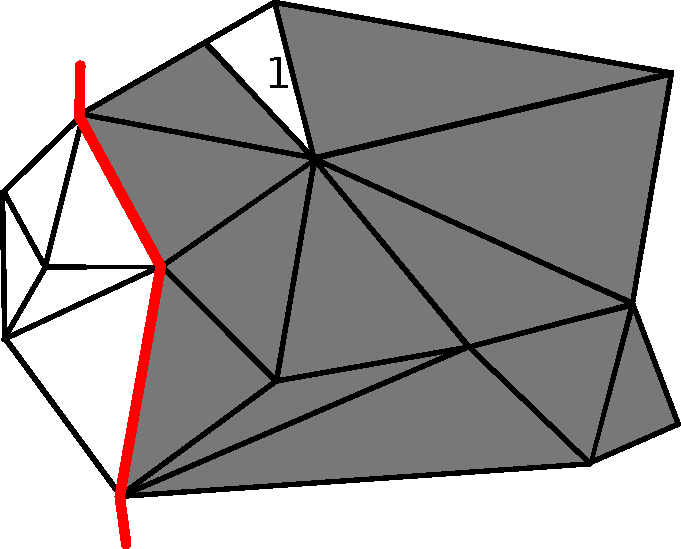
\includegraphics[width=0.24\columnwidth]{./img/ch_soa/incrementalGrowing00}&
  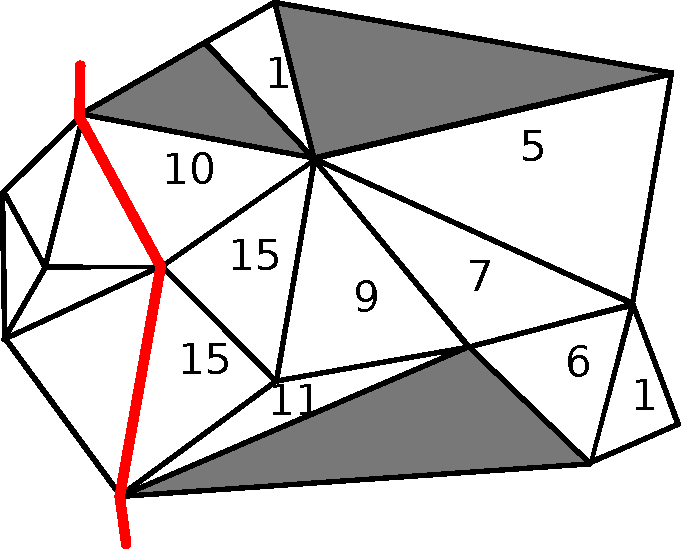
\includegraphics[width=0.24\columnwidth]{./img/ch_soa/incrementalGrowing01}&
  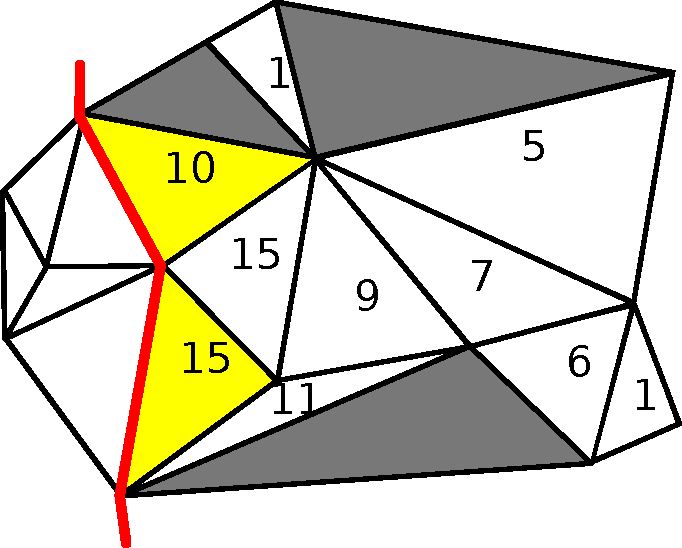
\includegraphics[width=0.24\columnwidth]{./img/ch_soa/incrementalGrowing02}&
  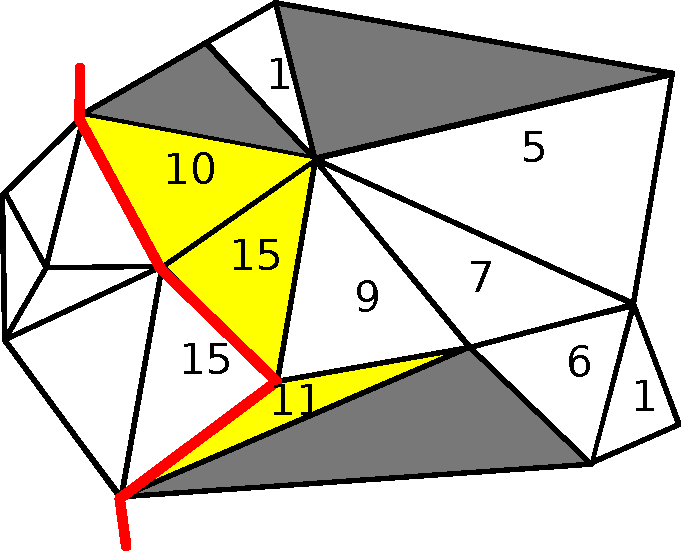
\includegraphics[width=0.24\columnwidth]{./img/ch_soa/incrementalGrowing03}\\
  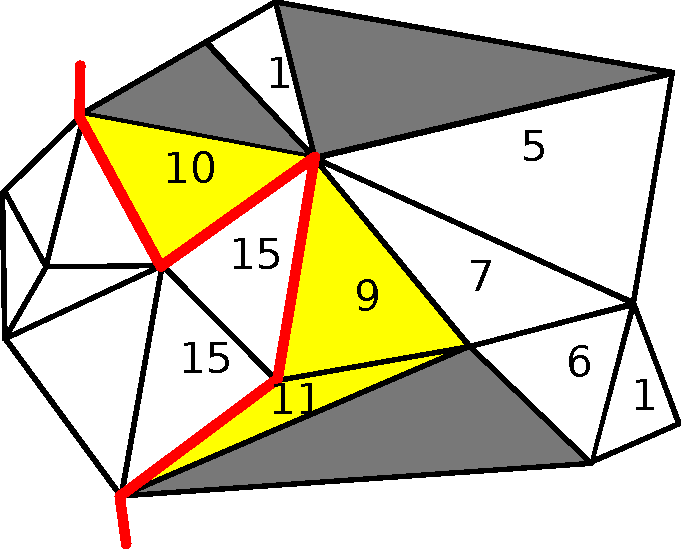
\includegraphics[width=0.24\columnwidth]{./img/ch_soa/incrementalGrowing04}&
  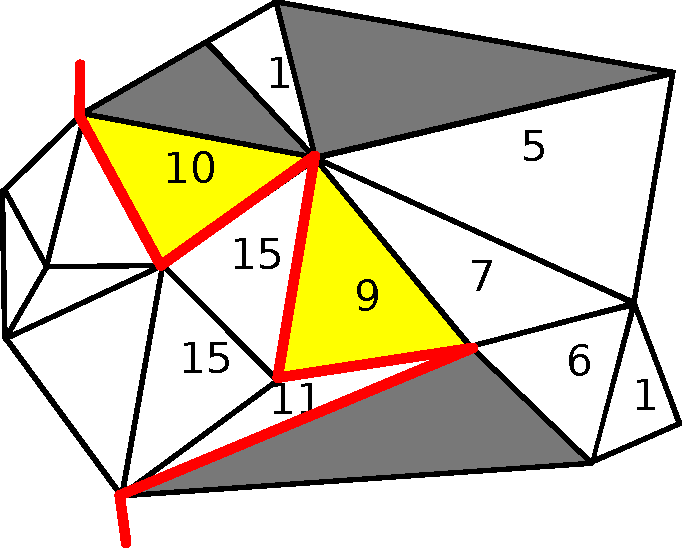
\includegraphics[width=0.24\columnwidth]{./img/ch_soa/incrementalGrowing05}&
  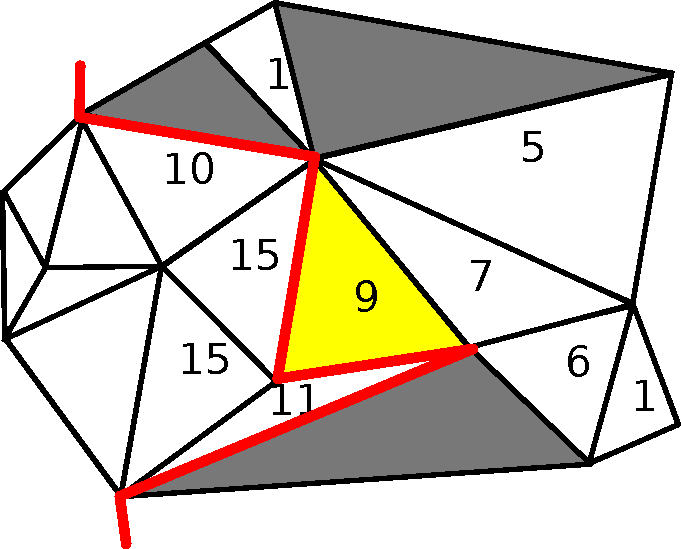
\includegraphics[width=0.24\columnwidth]{./img/ch_soa/incrementalGrowing06}&
  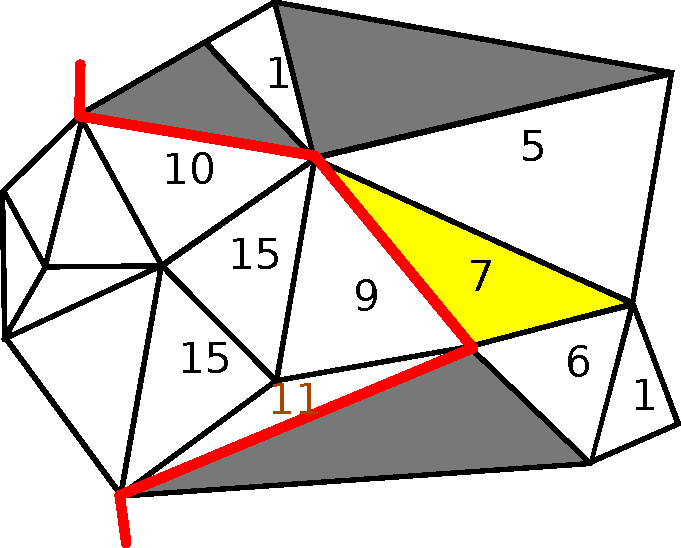
\includegraphics[width=0.24\columnwidth]{./img/ch_soa/incrementalGrowing07}\\
  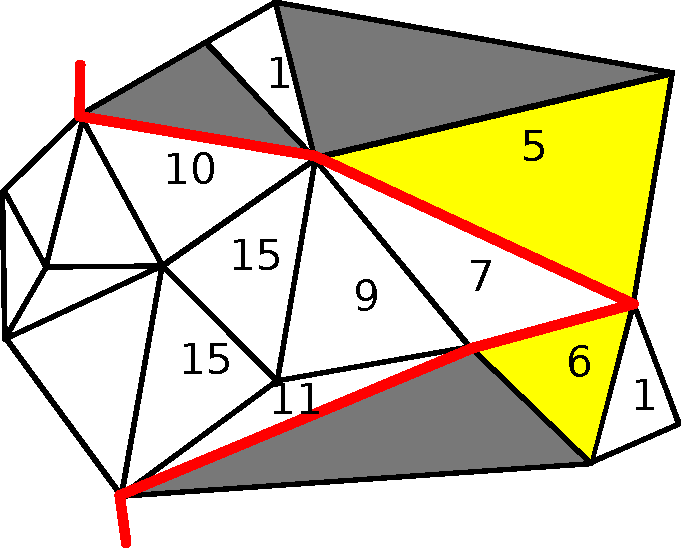
\includegraphics[width=0.24\columnwidth]{./img/ch_soa/incrementalGrowing08}&
  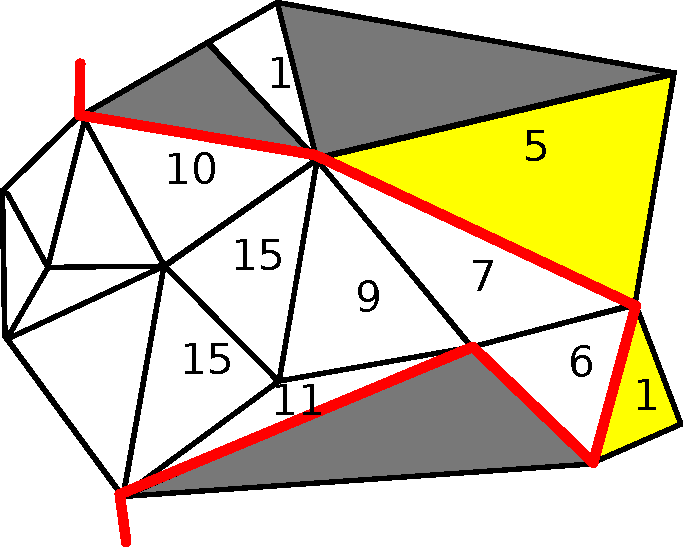
\includegraphics[width=0.24\columnwidth]{./img/ch_soa/incrementalGrowing09}&
  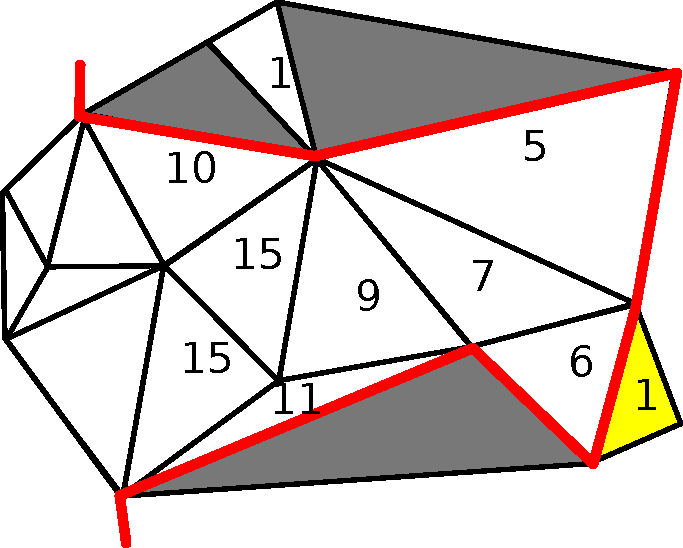
\includegraphics[width=0.24\columnwidth]{./img/ch_soa/incrementalGrowing10}&
  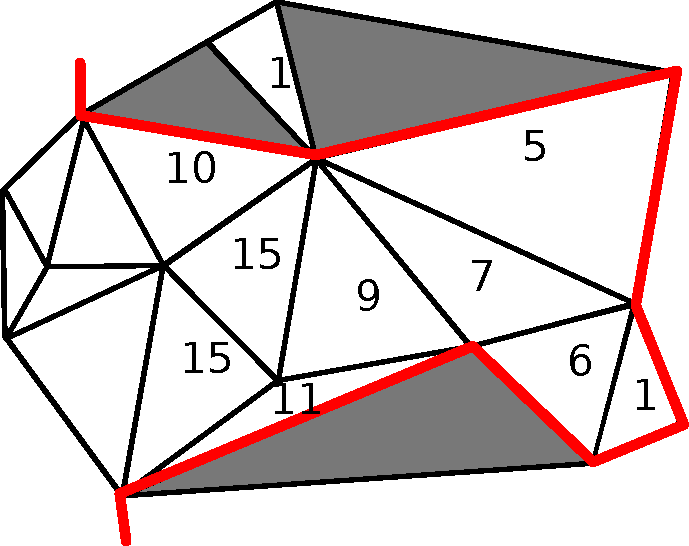
\includegraphics[width=0.24\columnwidth]{./img/ch_soa/incrementalGrowing11}\\
 \end{tabular}
 \caption{Example of manifold growing. The red line is the manifold, the numbers represent the number of ray intersections, the yellow the tetrahedra in the queue $Q$, in dark gray the triangles not intersected.}
 \label{fig:growing}
\end{figure}






Once the system is initialized, a new set of points $P_{t_k}$ is generated at $t_k= t_{\text{init}} + k*T_k$, where $k \in \mathbb{N^+}$ is the keyframe index and $T_k$ is the period. 
The insertion of each point $p\in P_{t_k}$ would cause the removal of a set $D_{t_k}$ of the tetrahedra that invalidates the Delaunay property (Figure \ref{fig:insertion}(a)); the surface $\delta (O_{t_k}) = \delta (O_{t_{k-1}} \setminus D_{t_k})$ is not guaranteed to be manifold anymore, or any other naive update of the triangulation potentially invalidates the manifoldness (Figure \ref{fig:insertion}(b)). 
To avoid this, the authors in \cite{litvinov_lhuillier_13} define a new list of tetrahedra $E_{t_k} \supset D_{t_k}$ (Figure \ref{fig:manifoldreconstruction}(b)) and they apply the so called \emph{Shrinking} procedure (Figure \ref{fig:manifoldreconstruction}(c)), i.e., the inverse of Growing: they subtract iteratively from $O_{t_{k-1}}$ the tetrahedra  $\Delta \in E_{t_k}$ keeping the manifoldness valid.
After this process, it is likely that $D_{t_k} \cap O_{t_k} = \emptyset$; however, in the case of $D_{t_k} \cap O_{t_k} \neq \emptyset$ the point $p$ is not added to the triangulation.
Otherwise, the point is added into the triangulation with the Point Addition step (Figure \ref{fig:manifoldreconstruction}(d)). 
Once all points in $P_{t_k}$ have been added (or dropped), then they apply the Ray Tracing  (Figure \ref{fig:manifoldreconstruction}(e)), and finally the Growing (Figure \ref{fig:manifoldreconstruction}(f)) similarly to the initialization procedure.


\begin{figure}[tp]
\centering
 \begin{tabular}{cc}
  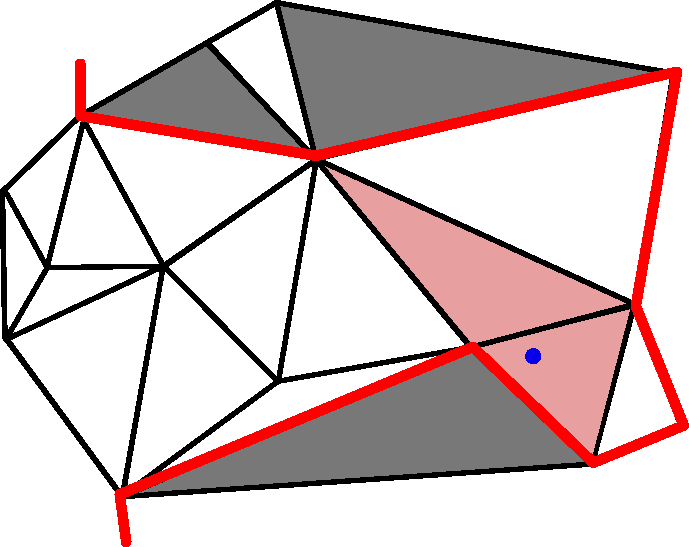
\includegraphics[width=0.45\columnwidth]{./img/ch_soa/pointIns01}&
  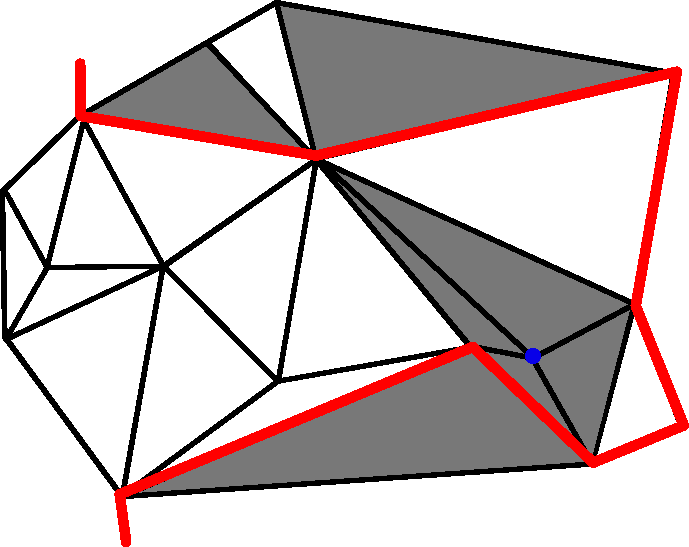
\includegraphics[width=0.45\columnwidth]{./img/ch_soa/pointIns02}\\
  (a)&(b)
 \end{tabular}
 \caption{Naive point insertion: a new point added to the triangulation needs re-triangulate a subset of tetrahedra; is not trivial to infer the new tetrahedra status (inside/outside) keeping the manifoldness valid.}
 \label{fig:insertion}
\end{figure}



\begin{figure}[tp]
\centering
 \begin{tabular}{ccc}
  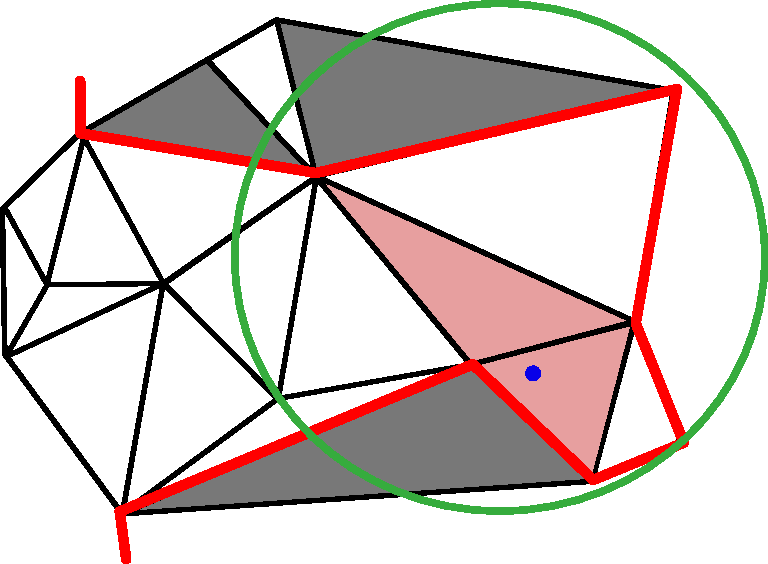
\includegraphics[width=0.33\columnwidth]{./img/ch_soa/manifoldRec01}&
  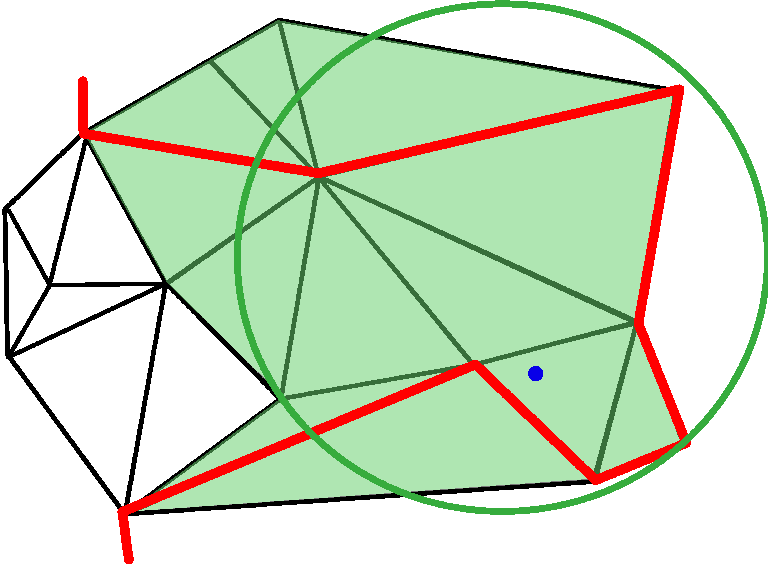
\includegraphics[width=0.33\columnwidth]{./img/ch_soa/manifoldRec02}&
  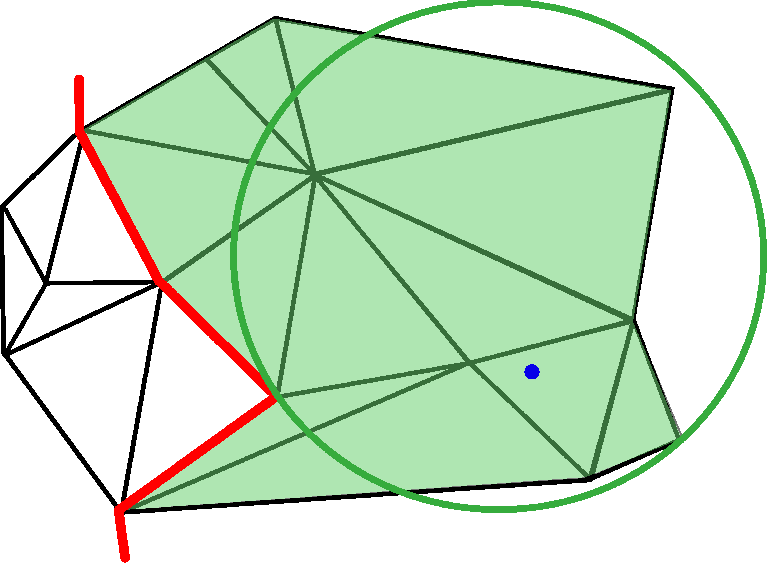
\includegraphics[width=0.33\columnwidth]{./img/ch_soa/manifoldRec03}\\
  (a)&(b)&(c)\\
  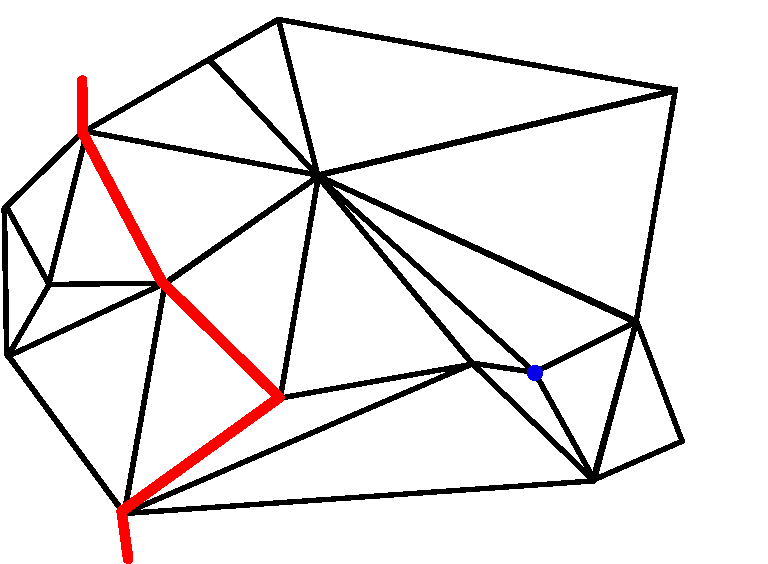
\includegraphics[width=0.33\columnwidth]{./img/ch_soa/manifoldRec04}&
  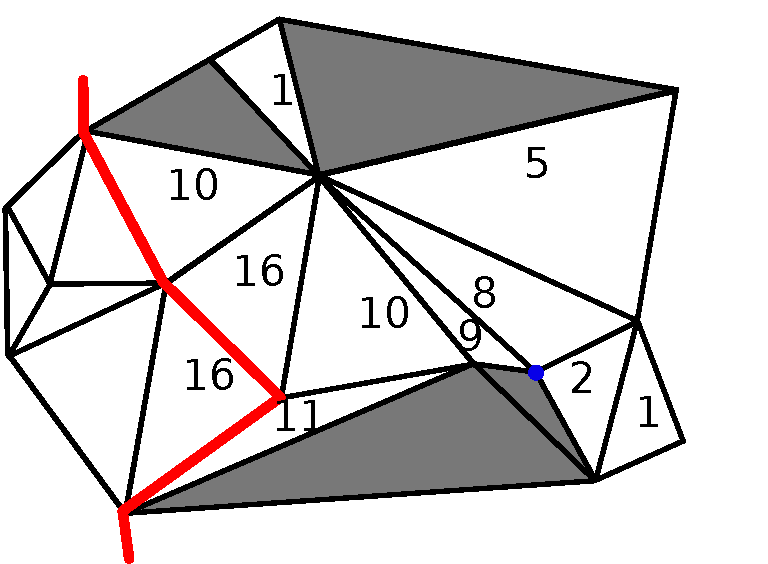
\includegraphics[width=0.33\columnwidth]{./img/ch_soa/manifoldRec05}&
  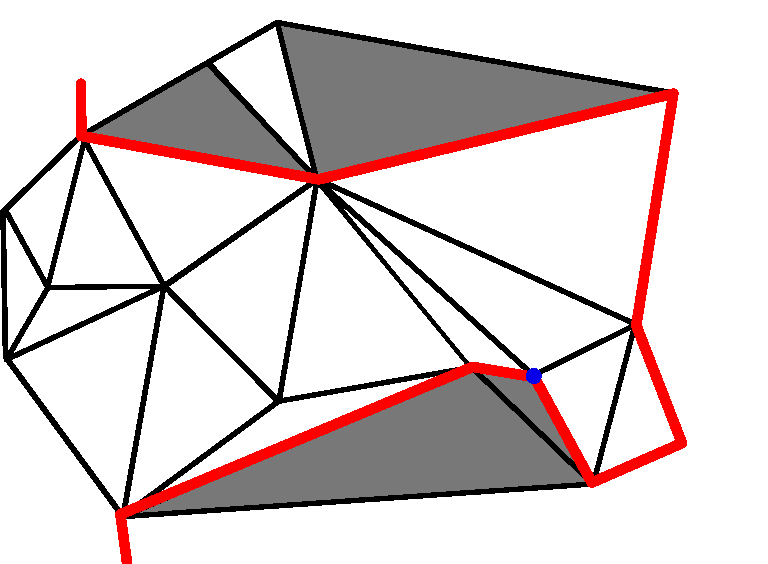
\includegraphics[width=0.33\columnwidth]{./img/ch_soa/manifoldRec06}\\
  (d)&(e)&(f)\\
  
 \end{tabular}
 \caption{Incremental manifold reconstruction steps: (a) a new point is estimated and it would invalidate the red tetrahedra (set $D_{t_k}$); (b) put a subset of this tetrahedra in $E_{t_k}$; (c) shrink the manifold; (d) add the point into the triangulation; (e) perform the ray tracing; (f) grow the manifold.}
 \label{fig:manifoldreconstruction}
\end{figure}

% Indeed, the very common approach to deal with a point moving in the triangulation, is to remove it and add it back in the new position \cite{cgal} (Fig. \ref{fig:moving}). 
% When we remove a point (the point A in Fig. \ref{fig:moving}(a)) and we want to keep the Delaunay property, we have to remove all the tetrahedra incident to that point (light red triangles in Fig. \ref{fig:moving}(b)); then, we add a new set of tetrahedra to triangulate the resulting hole (dark green triangles in \ref{fig:moving}(c)).
% When we add a new point into the triangulation  (the point B in Fig. \ref{fig:moving}(d)), a set of tetrahedra would conflict with it, \ie, the Delaunay property is broken (light red triangles in Fig. \ref{fig:moving}(d)); so, we remove this set of tetrahedra again (red triangles in Fig. \ref{fig:moving}(e)) and we add a new connected set that re-triangulate the hole (dark green triangles in Fig. \ref{fig:moving}(f)).
% Whenever a set of tetrahedra is replaced, we have to transfer conveniently the information about the visibility (matter or free space) of the removed tetrahedra to the new one. 
% In addition to this, we have to update the visibility of the tetrahedra crossed by a visibility ray from one camera to the moved point.
% For these reasons the update of the point position is computational demanding.


% \section{other sensors}



